%************************************************
\chapter{Resilience}\label{ch:resilience}
%************************************************
This chapter gives a brief introduction to Resilience in microservice architectures and show how Gatling load testing framework can be used for testing. This chapter also shows load testing scenarios against the PoC and describes the effects of using patterns??.\\

There are different categories of potential disruptions to system that create the need to implement the resilience in systems. In the figure \ref{ch:resilience} below the sources of disruptions is showed. 

\begin{figure}[bth]
	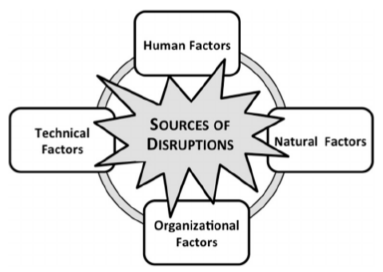
\includegraphics[width=0.7\linewidth]{gfx/resilience}
	\caption[routingtable]{Sources of disruptions} \label{fig:resilience}
\end{figure}   

\begin{itemize}
	\item Human Factor
	\begin{itemize}
		\item One of the common disruption is caused by human factors. The disruption in this case could be external attacks on the system, or just so simply as humans using the system.  
	\end{itemize}
	\item Natural Factors
	\begin{itemize}
		\item A infrequent influence on damaging the system caused by natural disaster, such as floods and hurricane. 
	\end{itemize}
	\item Organizational factors
	\begin{itemize}
		\item Another difficulty to be considered about disruption the system is organizational factors, such as the worker strikes.   
	\end{itemize}
	\item Technical Factors
	\begin{itemize}
		\item Technical difficulty need also to be considered in the system. It is common that system component fails, and need to be either replaced or to be repaired.   
	\end{itemize}	
\end{itemize}

All the factors described above need to be considered in the system to avoid disruption. 

To begin with the question really is "what is the actual definition of resilient?". There are different definitions and they strongly depends upon the context it is used inside. In the sense of microservices the definition could sound like so:\\
\textit{The power or ability of a microservice to return to the its original form, after being affected by failures according to unusual scenarios.}

Thus, from the definition above the resilient system should be able to cope with problem and at the same time be fast to recover. 

In the case of microservices the services are highly decoupled. By the isolation of microservices makes them independent from each other, so in the case of that one of them fails the other services do not stop working. By having the services decoupled in the system we get a lot of resilience into applications, thus they get ability to handle disruptions. 

This isolation of simple small services makes them independent from each other, so that when one fails the others don’t stop working.   

\section{PoC load tests}
To load-test the developed PoC containers a tool called Gatling is used. Gatling gives you the ability to record a test scenario for your microservices using web-browsers. A Scala file can be generated from the recorded scenario. Following is a code snippet of the generated Scala code for the PoC which was modified to run 100 times instead of a single run: \begin{lstlisting}[frame=single, ]
val uri1 = "http://192.168.1.11"

val scn = scenario("RecordedSimulation")
.exec(http("request_0")
.get("/search/?w=berry"))
.pause(4)
...

setUp(scn.inject(atOnceUsers(100))).protocols(httpProtocol)
\end{lstlisting}

To run the test, a script called \textit{gatling.sh} has to be called. The test results is builed as a HTML-site with different kinds of charts illustrating response time distribution, response time percentiles, requests/responses rates, and others. Figure \label{fig:responseTimeDistribution} shows a chart with the response time distribution of the PoC load test. It is clear by the chart that all the request have passed and that the majority of the responses have a time less than 250 ms.

\begin{figure}[bth]
	\centering 
	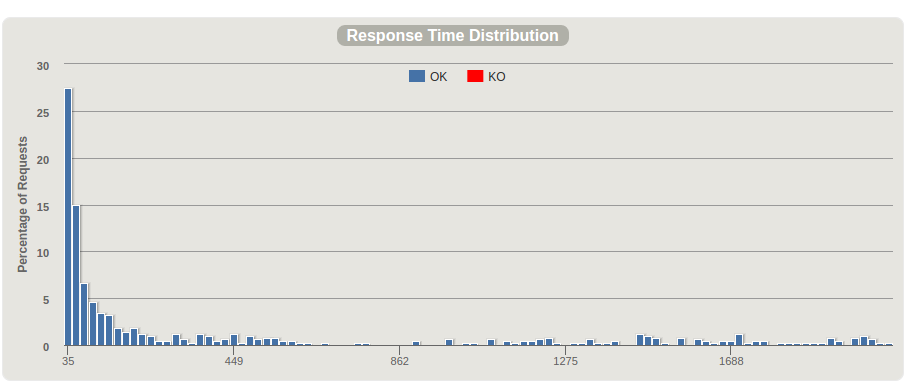
\includegraphics[width=1\linewidth]{gfx/responseTimeDistribution}
	\caption[responseTimeDistribution]{Response time distribution of the PoC load test} \label{fig:responseTimeDistribution}
\end{figure}